\chapter{Introduction}\label{ch:introduction}
\graphicspath{{../Figures/10-introduction/}{figs/10-introduction/}}

The overall goal of the bipedal robot project in the Agile and Adaptive Robotics Lab at Portland State University is to create a high-fidelity biomimetic humanoid robot actuated by artificial muscles and controlled by a synthetic nervous system (SNS). This dissertation develops tools needed to pursue that goal. The work starts with characterizing actuator force and predicting joint torque and proceeds to organizing sensory-afferent evidence and developing tools for constructing and testing neural controllers in coupled mechanical models. The following sections explain why these four contributions are needed, position them within the robot project, state the research objectives, and describe the dissertation's organization.

\section{Motivation}

The motivation for biomimetic robot design tools is grounded in two complementary halves of an iterative design loop. The first half draws on principles from biomechanics and neuroscience to develop robots with improved autonomy, balance, and adaptability in unstructured terrain \citep{frey_legged_2026, ha_learning_2025, ijspeert_amphibious_2020}. Compliant actuation and biologically inspired neural control also offer potential improvements in locomotor energy economy. The second half uses these robots as controllable physical models to investigate biological movement, including the mechanisms underlying motion generation, internal forces, and neural control \citep{asano_design_2017, hitzmann_anthropomorphic_2018}. Robotic platforms allow researchers to systematically manipulate actuator properties, mechanical configurations, and sensory pathways under repeatable conditions, including interventions that would be impractical or unethical in human participants. They therefore complement animal studies and numerical models by enabling the coupled mechanical and neural contributions to movement to be investigated experimentally \citep{shin_constructive_2018, goldsmith_investigating_2021}. This iterative process is illustrated by \citet{ijspeert_swimming_2007} using a salamander robot, in which biological evidence informed a spinal cord model, and subsequent robotic experiments generated predictions that were examined in biological preparations. This reciprocal approach also has potential applications in the development of prosthetic and orthotic devices. In these ways, biological understanding informs robotic design, while robotic experiments provide new hypotheses and insights that can be returned to biology. 

The first mechanical design consideration is to select artificial muscles that can meet the robot joints' torque requirements within the available space. The McKibben-style braided pneumatic actuators (BPAs) used here combine low mass, high force-to-weight ratio, and intrinsic compliance with a force--length curve that qualitatively resembles that of skeletal muscle \citep{liang_comparative_2020, hunt_modeling_2017}. Our initial work with Festo BPAs showed that at shorter resting (uninflated) lengths, they delivered less force and contraction than what the manufacturer specifies. Existing empirical models describe useful pressure--contraction relationships \citep{sarosi_comparative_2017, martens_modeling_2017, hunt_modeling_2017}, but did not capture this relationship between resting length and force output. Therefore, I built a jig to perform isometric force experiments with Festo BPAs and collect data to further characterize this relationship. This data enabled the development of actuator force models that account for resting length, pressure, and contraction. The work in Chapter~\ref{ch:muscles} describes this process and the developed model.

The next mechanical design consideration is predicting joint torque of an assembled robot. When an artificial muscles pulls on a limb segment, it creates torque about the joint. This torque is what moves the body through space, causing the limbs to interact with objects and the ground. The artificial muscle force is transmitted to the skeleton through mounting brackets and artificial tendons. Brackets and fixtures can deflect under load, tendons can stretch, and contact with the skeleton bends an actuator. All this changes the force and torque that an artificial muscle applies to the limb. This compliance and actuator bending can therefore cause rigid-body predictions of torque typically used in robotic models to differ from actual torque. Initial tests showed that joint torque and the usable range of motion (RoM) on a knee joint were lower than predicted. I therefore built an isometric knee-torque test jig to develop a model of how the artificial muscle interacts with limb, and better predict the expected joint torque. The improved model was then used to design and test artificial musculotendon routes that can meet or exceed their human-muscle torque equivalents. The details of this process are described in (Chapter~\ref{ch:torque}).

In addition to the accurate biomechanical model of the human body, the goals of the bipedal robot project include the use of an underlying neural controller that mimics the human nervous system.  To build such a model, it is necessary to gather and curate a collection of material on how the nervous system is organized and how sensory input influences neural activity and movement. Unfortunately, there is not a complete understanding of this, no comprehensive view has been written or collected from scientific papers. Our understanding of neural control is distributed across species, preparations, and experimental protocols \citep{van_de_crommert_review_1998, windhorst_muscle_2007, windhorst_spinal_2022}. Therefore, I developed the Sensory Afferent Database (SADb) to aid in organizing the literature on the subject into a searchable resource linked to its sources. Chapter~\ref{ch:database} provides an overview of how the SADb was developed, how it is organized, and features that can be used to sort and understand the underlying material.

The sensory pathways documented in the database suggest how the nervous system uses feedback from the legs to coordinate movement. To simulate what those pathways contribute, it is possible to combine a neural circuit model with the mechanical model of the body it controls. The circuit activates muscles, their forces move the joints, and the resulting changes in muscle stretch and load feed back to the circuit and shape its next commands. The robot’s artificial muscles differ from human muscles in how much force they produce and where they pull on the skeleton. A circuit that coordinates the legs of the human model will therefore produce a different movement in the robot model, and that movement will change the sensory feedback the circuit receives. To measure the effect of the mechanics, I wanted to repeat the same experiment on both models with the controller held fixed. I also wanted to test changes to the controller while keeping the mechanical model fixed. Our first neuromechanical model ran slowly, and we tuned its controller by hand, making a series of these comparisons impractical. I therefore developed tools to build circuits graphically, automate their tuning, and run those comparisons on a human musculoskeletal model and on models built from our robot's mechanical design (Chapter~\ref{ch:sns}). With human movement as a reference, the new system can simulate how changing a sensory connection or moving an artificial muscle attachment affects a mechanical model's coordination.

\section{The Biomimetic Humanoid Robot Project}\label{sec:project}

The Portland State University robot project currently focuses on a lower-body platform representing the body from the lumbar spine down, with a human-scale skeleton, artificial tendons, BPAs, and biomimetic joint mechanisms. Preserving human-like joint motion and musculotendon organization provides a mechanical basis for investigating interactions between biomechanics and neural control. These anatomical relationships matter because joint geometry and muscle routing determine how actuator forces produce movement and how movement generates sensory feedback..

The project uses OpenSim's Gait2392 musculoskeletal model as a benchmark for human joint motion, musculotendon geometry, and torque-generating capacity \citep{delp_opensim_2007, bolen_bipedal_2019}. Gait2392 includes 92 musculotendon actuators and 23 degrees of freedom (DoF), six of which describe the position and orientation of the pelvis in space. I developed the robot's kinematic design for my master's project. The design includes 17 internal joint DoF, with 27 musculotendon actuator units on each side \citep{bolen_bipedal_2019, bolen_determination_2019}. The associated computational tools allow the robot's muscle lengths, moment arms, and joint torques to be compared with corresponding human-model predictions. These comparisons provide a basis for assessing how design changes affect the robot's ability to reproduce selected biomechanical functions.

The physical implementation combines commercially available Festo BPAs and artificial tendons with three-dimensional printing and machining. These technologies allow human-scale skeletal geometry, custom actuator attachments, and biomimetic joint mechanisms to be constructed and revised using available components and fabrication methods. The four-bar knee linkage developed by \citet{steele_development_2017, steele_biomimetic_2018, steele_biomimetic_2018-1} incorporates a migrating instantaneous center of rotation, reproducing an important feature of human knee motion that influences muscle leverage. The project therefore examines how selected anatomical and mechanical relationships can be realized within the force, contraction, and packaging limits of available artificial muscles.

The platform provides a foundation for progressive development of its mechanical, neural-control, and sensing capabilities. Actuator-placement optimization can extend the methods developed for the knee to other joints, selecting actuator lengths and musculotendon routes that meet joint-torque targets over the required RoM. Integrating a synthetic nervous system with the physical robot would enable sensory feedback and biologically inspired neural circuits to coordinate its artificial muscles, providing a platform for investigating neuromechanical interactions. Longer-term extensions could incorporate machine vision to provide information about terrain and obstacles, together with GPU-based computation to support more demanding perception and control tasks. These capabilities would expand the range of movements and environments that the robot could be used to investigate.

\section{Research Objectives}\label{sec:objectives}

The four research objectives define the contributions of this dissertation:

\begin{enumerate}
    \item \textbf{Characterize the isometric force of Festo BPAs} with uninflated diameters ($\diameter$) of \qtylist{10;20}{\mm} across resting lengths, contractions, and pressures; develop resting-length-dependent maximum-force and normalized force--strain--pressure models; and compare their predictions with existing models (Chapter~\ref{ch:muscles}).
    \item \textbf{Validate and improve isometric knee-torque prediction} on pinned and biomimetic four-bar knees; identify and validate corrections for length offsets, effective series compliance, and actuator bending; and use the improved model to redesign and test routes against selected human-muscle torque targets (Chapter~\ref{ch:torque}).
    \item \textbf{Develop a searchable sensory-afferent literature database}, the Sensory Afferent Database (SADb), by curating published afferent properties, pathways, and their experimental contexts (Chapter~\ref{ch:database}).
    \item \textbf{Develop tools for constructing and testing neuromechanical models} that couple neural controllers to human and BPA-actuated robot mechanics; connect graphical model construction with automated tuning and experiments; and verify representative circuit responses, implementation agreement, and neural--mechanical signal exchange (Chapter~\ref{ch:sns}).
\end{enumerate}

\section{Dissertation Organization}\label{sec:organization}
\begingroup
\clubpenalty=10000
\widowpenalty=10000

The dissertation develops the mechanical and neural foundations of the humanoid robot through four connected studies. The mechanical studies examine actuator force and joint torque, while the neural studies address physiological evidence and tools for constructing and testing neuromechanical models. The chapter sequence develops these contributions from their scientific background through their methods, evidence, and implications for robot development. Figure~\ref{fig:roadmap} summarizes their relationships within the broader research program.

Chapter~\ref{ch:background} establishes the concepts needed to connect mechanical design with neural control. It reviews biomimetic robots, actuation, BPA behavior, and lower-limb biomechanics as the basis for interpreting the mechanical experiments. Locomotor control and sensory feedback provide the biological context for the neural models, followed by the tools used for neuromechanical simulation. The chapter closes with the scientific and ethical rationale for robotic experiments.

Chapter~\ref{ch:muscles} presents the isometric BPA characterization study adapted from my publication \citep{bolen_2026}. Measurements across resting lengths, contractions, and pressures are used to develop the maximum-force and normalized force--strain--pressure relationships. Comparisons with existing models assess their predictions against the measured actuator behavior, and the discussion examines their implications for actuator selection and the analogy with biological muscle. The chapter thus connects empirical characterization to a force model that is subsequently used in the knee-torque study and the BPA-actuated neuromechanical simulations.

Chapter~\ref{ch:torque} extends the analysis from actuator force to the torque transmitted through the knee mechanics. Experiments on pinned and biomimetic knees evaluate the effects of joint kinematics, compliance, and actuator wrapping on torque prediction. Corrections for length offsets, effective series compliance, and bending are identified and evaluated using separate tests. The improved model is then used to select actuator lengths and redesign musculotendon routes. Physical tests of the redesigned configurations complete the connection between actuator characterization, mechanical design, and measured performance against selected human-muscle torque targets.

Chapter~\ref{ch:database} turns to the physiological evidence required for sensory-feedback selection. It presents SADb as a searchable collection linking afferent properties and pathways to the experimental conditions and sources from which they were reported. The chapter explains the curation and classification of these records, evaluates AI-assisted screening of candidate additions, and examines the collection's coverage. The discussion relates the collection's coverage and the context of its sources to its use in neuromechanical modeling.

Chapter~\ref{ch:sns} develops the capabilities needed to turn neural-control hypotheses and mechanical models into executable experiments. The initial AnimatLab controller-transfer attempt introduces the practical problem of adapting a circuit to different mechanics and sensory conditions. The chapter follows human-model conversion from OpenSim to MuJoCo and graphical robot-model construction through SNS-Simscape. Command and sensory-signal exchange, graphical inspection, staged tuning, and automated experiments are developed as complementary parts of this workflow. Representative circuit tests, implementation comparisons, and coupled-model demonstrations accompany the construction steps, establishing the capabilities available for subsequent controller and hardware investigations.

Chapter~\ref{ch:overall} integrates the four studies within the broader humanoid robot program. It considers the contributions and their associated research opportunities within a common design workflow. The mechanical discussion connects actuator characterization and joint-torque prediction to dynamic testing and further BPA routing optimization. The neural discussion connects continued literature curation and simulation experiments to sensory integration, higher-level control, and physical hardware, relating the established evidence to the next stages of the project.

Chapter~\ref{ch:conclusion} states the conclusions in relation to the four research objectives. It draws together the experimental basis for actuator and knee design, the means of locating and interpreting sensory-afferent evidence, and the capabilities demonstrated by the neuromechanical tools. The chapter closes by relating these outcomes to the larger aim of using a biomimetic humanoid to investigate interactions between mechanical structure and neural control.


\par
\endgroup
\begin{figure}[htbp]
\centering
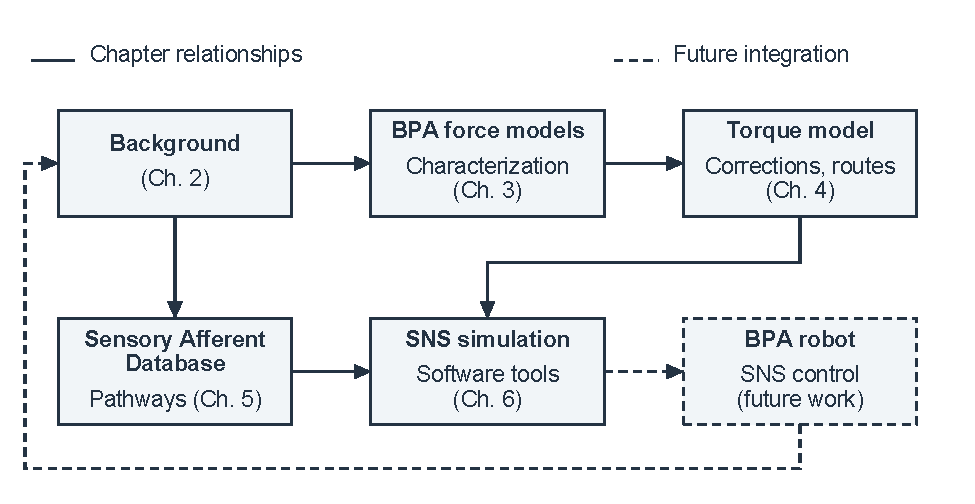
\includegraphics[width=\textwidth]{roadmap.pdf}
\caption[Dissertation roadmap]{Relationships among the dissertation studies and their proposed integration in the physical robot.
}
\label{fig:roadmap}
\end{figure}

